  
\documentclass{beamer}
\usepackage{listings}
\usepackage{graphicx}
\usepackage{epstopdf}
\usepackage{hyperref}

\lstset{
		tabsize=4,
        basicstyle=\scriptsize,
        %captionpos=b,
        %upquote=true,
        aboveskip={1.5\baselineskip},
        columns=fixed,
        showstringspaces=false,
        extendedchars=true,
        breaklines=true,
        prebreak = \raisebox{0ex}[0ex][0ex]{\ensuremath{\hookleftarrow}},
        frame=tRBl,
	    %frameround=tttf,
	    numbers=left,
	    numberstyle=\tiny,
	    numbersep=5pt,
        showtabs=false,
        showspaces=false,
        showstringspaces=false,
        identifierstyle=\ttfamily,
        keywordstyle=\color[rgb]{0,0,1},
        commentstyle=\color[rgb]{0.133,0.545,0.133},
        stringstyle=\color[rgb]{0.627,0.126,0.941},
        aboveskip=5pt
}

\usetheme{AnnArbor}
\usecolortheme{beaver}
\setbeamertemplate{note page}[plain]
\begin{document}

\title{Introduction to Web Development}
\subtitle{using Sinatra}
\author[Konstantinos Karasavvas]{Konstantinos Karasavvas} %\\{\small Software Architect and Engineer}}

\institute{CITY College}
\date{\today} 

\begin{frame}
  \titlepage
\end{frame}

\begin{frame}
\setcounter{tocdepth}{2}
\frametitle{Table of contents}
\tableofcontents
\end{frame} 





\section{More Sinatra}

\subsection{Multiple Environments} 
\begin{frame}\frametitle{Multiple Environments} 
  \begin{itemize}
    \item Different Environments, typically: 
    \begin{itemize}
      \item development
      \item test
      \item production
    \end{itemize}

    \item Database adaptors
    \item Testing libraries
    \item ...        
  \end{itemize}
\end{frame}



\begin{frame}[fragile]\frametitle{Multiple Environments: Gemfile} 

  \lstinputlisting[language=ruby]{code/proj1/Gemfile}
  
  \begin{lstlisting}[language=bash, escapechar={^}]
$ bundle install
...
  \end{lstlisting}

\end{frame}




\begin{frame}[fragile]\frametitle{Multiple Environments: Tiny App} 

  \lstinputlisting[language=ruby, lastline=13]{code/proj1/user_app8.rb}
  
  \lstinputlisting[language=ruby]{code/proj1/models/users.rb}

\end{frame}






\begin{frame}[fragile]\frametitle{Multiple Environments: Tiny App, cont.} 

  \lstinputlisting[language=ruby]{code/proj1/config8.ru}

  \begin{lstlisting}[language=bash, escapechar={^}]
$ rackup -E production config8.ru
...
  \end{lstlisting}
  
  \begin{lstlisting}[language=bash, escapechar={^}]
$ rackup config8.ru
...
  \end{lstlisting}
  
\end{frame}






\subsection{Logging} 
\begin{frame}\frametitle{Logging}
 
  \begin{itemize}
  
    \item Why?
    \begin{itemize}
      \item Diagnostic (something went wrong)
      \item Audit (statistic analysis)
    \end{itemize}

    \item Levels
    \begin{itemize}
      \item \texttt{debug}
      \item \texttt{info}
      \item \texttt{warn}
      \item \texttt{error}
      \item \texttt{fatal}
    \end{itemize}

  \end{itemize}

\end{frame}



\begin{frame}[fragile]\frametitle{Simple Logging: Tiny App}

  \begin{lstlisting}[language=ruby, escapechar={^}]
  # ...
  
  get "/hello_form" do
    logger.info "Entered /hello_form route"
    @title = "Hello Stored User"
    haml :form2, :layout => true
  end 
  
  # ...
  \end{lstlisting}

\end{frame}




\begin{frame}[fragile]\frametitle{File Logging: Tiny App} 

  \begin{itemize}
    \item Add a logging library to our \texttt{Gemfile}
  \end{itemize}
  \begin{lstlisting}[language=ruby, escapechar={^}]
# ...
gem 'log4r'
# ...
  \end{lstlisting}
  
  \begin{lstlisting}[language=bash, escapechar={^}]
$ bundle install
...
  \end{lstlisting}



\end{frame}




\begin{frame}[fragile]\frametitle{File Logging: Tiny App, cont.} 

  \lstinputlisting[language=ruby]{code/proj1/config9.ru}


  \begin{lstlisting}[language=bash, escapechar={^}]
$ mkdir logs
  \end{lstlisting}


\end{frame}



\begin{frame}[fragile]\frametitle{File Logging: Tiny App, cont.} 

  \begin{lstlisting}[language=bash, escapechar={^}]
  # ...
  
  get "/hello_form" do
    logger = Log4r::Logger["app"]
    logger.info "Entered /hello_form route"
    @title = "Hello Stored User"
    haml :form2, :layout => true
  end 
  
  # ...
  \end{lstlisting}

  \begin{lstlisting}[language=bash, escapechar={^}]
$ cat logs/20130731-233135.log 
 INFO app: Entered /hello_form route
  \end{lstlisting}

\end{frame}



\subsection{Sessions} 
\begin{frame}\frametitle{Sessions}
 
  \begin{itemize}
  
    \item HTTP is stateless
    \item Sessions allow us to have state between requests
    \item E.g., the app should \textit{remember}:
    \begin{itemize}
      \item user logins
      \item user adding items in the shopping cart
      \item ...
    \end{itemize}

    \item And has to remember them for multiple clients/conversations
    
    \item Implementation
    \begin{itemize}
      \item HTTP session token
      \item Via cookies or GET/POST back to the server
    \end{itemize}

  \end{itemize}

\end{frame}




\begin{frame}\frametitle{Sessions, cont.}
 
  \begin{center}
    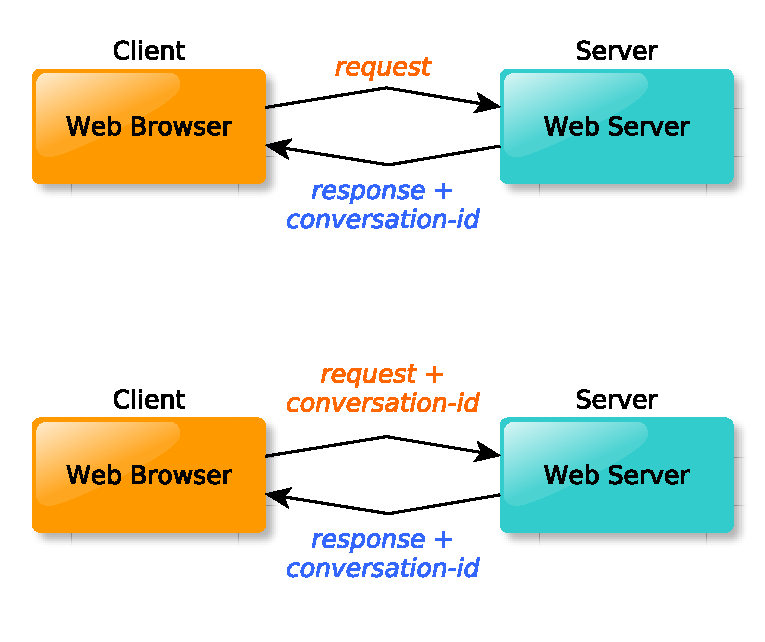
\includegraphics[scale=0.5]{diagrams/sessions.pdf}  
  \end{center}

\end{frame}



\begin{frame}\frametitle{Sessions: Example}
 
    \lstinputlisting[language=ruby]{code/sessions.rb}
 
\end{frame}




\subsection{MIME Types and Attachments} 
\begin{frame}\frametitle{MIME Types and Attachments}
 
  \begin{itemize}
  
    \item Multipurpose Internet Mail Extensions (MIME)
    \begin{itemize}
      \item initially for emails
      \item used to describe the content type
    \end{itemize}

    \item Widely used, e.g. in HTTP
    
  \end{itemize}

\end{frame}





\begin{frame}\frametitle{Sessions: Example 1}
 
    \lstinputlisting[language=ruby]{code/mime_types.rb}
 
\end{frame}





\begin{frame}\frametitle{Sessions: Example 2}
 
    \lstinputlisting[language=ruby]{code/mime_types2.rb}
 
\end{frame}




\begin{frame}\frametitle{Sessions: Example 3}
 
    \lstinputlisting[language=ruby]{code/mime_types3.rb}
 
\end{frame}




\subsection{Error Handling} 
\begin{frame}\frametitle{Error Handling}
 
  \begin{itemize}

    \item HTTP Status Codes
    \begin{itemize}
      \item 1xx: Informational
      \item 2xx: Success
      \item 3xx: Redirection
      \item 4xx: Client Error
      \item 5xx: Server Error
    \end{itemize}
  
    \item Example error codes
    \begin{itemize}
      \item 403: Forbidden
      \item 404: Not Found
      \item 500: Internal Server Error
      \item ...
    \end{itemize}

    \item Our app should properly handle those errors
    
  \end{itemize}

\end{frame}



\begin{frame}\frametitle{Error Handling: Example 1}
 
    \lstinputlisting[language=ruby]{code/errors.rb}
 
\end{frame}





\begin{frame}\frametitle{Error Handling: Example 2}
 
    \lstinputlisting[language=ruby]{code/errors2.rb}
 
\end{frame}




\subsection{More Configuration} 
\begin{frame}[fragile]\frametitle{More Configuration}
 
  \begin{lstlisting}[language=ruby, escapechar={^}]
configure do
  set :environment, ENV["RACK_ENV"]
  enable :logging
  set :sessions, true
  set :public_folder, "public"
  disable :show_exceptions
  set :root, "."
  set :static
  set :views, "views"
  
  # Custom  
  set :key, "value"
end
  \end{lstlisting}
 
  \begin{lstlisting}[language=ruby, escapechar={^}]
get "/" do
  settings.key
end
  \end{lstlisting}

\end{frame}




\subsection{Filters} 
\begin{frame}\frametitle{Filters}
 
    \lstinputlisting[language=ruby]{code/filters.rb}
 
\end{frame}




\begin{frame}[fragile]\frametitle{Filters}

  \begin{lstlisting}[language=bash, basicstyle=\tiny, escapechar={^}]
$ ruby filters.rb 
[2013-08-01 20:22:23] INFO  WEBrick 1.3.1
[2013-08-01 20:22:23] INFO  ruby 1.9.3 (2012-12-25) [x86_64-linux]
== Sinatra/1.4.3 has taken the stage on 4567 for development with backup from WEBrick
[2013-08-01 20:22:23] INFO  WEBrick::HTTPServer#start: pid=8492 port=4567
I, [2013-08-01T20:22:46.326070 #8492]  INFO -- : Entered 'before' block.
I, [2013-08-01T20:22:46.326424 #8492]  INFO -- : Entered '/' route.
I, [2013-08-01T20:22:46.326644 #8492]  INFO -- : Entered 'after' block.
127.0.0.1 - - [01/Aug/2013 20:22:46] "GET / HTTP/1.1" 200 40 0.0054
localhost - - [01/Aug/2013:20:22:46 EEST] "GET / HTTP/1.1" 200 40
- -> /
  \end{lstlisting}

\end{frame}


\end{document}
